\documentclass{report}

\usepackage{../../../../../LaTeX/marzstyle}

\author{Marcel \textsc{Zauder} 16-124-836 \\
	Pascal \textsc{Gerig} 16-104-721}

\runningheads{Concurrency}{Exercise 03}

\setcounter{chapter}{3}

\begin{document}
	\section{Several Questions}
	\startsection
		\begin{enumerate}[a)]
			\item \textit{What does a safety property do in FSP?} \\
			A safety property in FSP is an expression that defines which actions are allowed. Actions that were not specified within a safety property are considered to lead to an \textsc{error}.
			\item \textit{Is the busy-wait mutex protocol fair? Justify your answer.} \\
			We will consider the implementation of slide 19 of the lecture. \\
			Yes, it is, because assuming that P1 wants to enter the critical section, but can't because P2 is currently in the CS. Therefore \textit{enter1} is \textsc{true}, \textit{enter2} is \textsc{true}, and \textit{turn} is P2. P1 is therefore currently in the busy wait loop. Eventually P2 will terminate its CS, assuming that none of the processes crashes, otherwise no progrss could be made if P2 crashes while in the CS, and set \textit{enter2} to false. Therefore P1 will leave the busy loop and enter the CS. If P2 wants to enter the CS again it will wait until P1 has finished its CS. \\
			For an abitrary implemenentation of a busy-wait mutex this would sometimes not be the case.
			\item \textit{Can you ensure safety for shared data in concurrent programs without using any kind of locks?} \\
			It would be possible if one can ensure that all operations that access the shared data are atomic. For example in Java there are atomic data types already implemented, e.g. AtomicInteger or ConcurrentLinkedQueue. With these types read and write operations are atomic (CompareAndSet operations are used to modify, change the data). 
			\item \textit{The Java language designers decided to implement concurrency based on monitors. What is the main reason behind this decision?} \\
			Because every object in Java can be logically associated with a monitor, implementing concurrency with these is much easier to use instead of always having to instantiate a lock or semaphore.
		\end{enumerate}
	\closesection
	
	\section{FSP Processes}
	\startsection
		As shown below with the LTSA tool both process definitions are not equal, because in T1 \textit{c} is a shared action, whereas in T2 it is a seperate action for both traces. \\
		\begin{tabular}{ccc}
			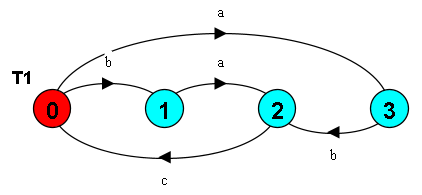
\includegraphics[scale=0.6]{T1.png} && 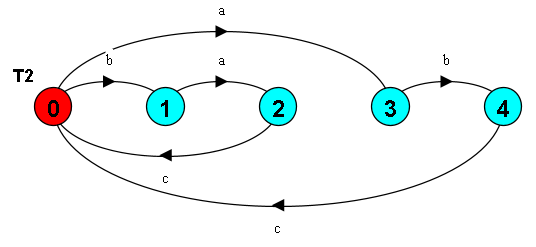
\includegraphics[scale=0.6]{T2.png} \\
			R = (a->c->R). && T2 = (a->b->c->T2 | b->a->c->T2). \\
			S = (b->c->S). \\
			||T1 = (R || S).
		\end{tabular}
	\closesection
	
	\newpage	
	
	\section{FM Radio}
	\startsection
		The radio is implemented as follows:
		\startsubsection
			\begin{minted}{bash}
const MAXFREQ = 10
const BOTFREQ = 1

RADIO = OFF,
OFF = (on -> HIGHESTFREQ | reset -> OFF | scan -> OFF),
HIGHESTFREQ = (off -> OFF | scan -> VALID[MAXFREQ] | scan -> INVALID[MAXFREQ] | 
	reset -> HIGHESTFREQ),
VALID[n:1..MAXFREQ] = (off -> OFF | lock -> LOCK[n] | reset -> HIGHESTFREQ),
INVALID[n:1..MAXFREQ] = (off -> OFF | when (n > BOTFREQ) scan -> VALID[n-1] | 
	when (n > BOTFREQ) scan -> INVALID[n-1] | 
	when (n == BOTFREQ) end -> NOTFOUND | reset -> HIGHESTFREQ),
LOCK[n:1..MAXFREQ] = (off -> OFF | when (n > BOTFREQ) scan -> VALID[n-1] | 
	when (n > BOTFREQ) scan -> INVALID[n-1] | 
	when (n == BOTFREQ) end -> NOTFOUND | reset -> HIGHESTFREQ),
NOTFOUND = (off -> OFF | reset -> HIGHESTFREQ | scan -> NOTFOUND).
			\end{minted}
		\closesection
		The idea with our implementation is that we can define the highest and lowest frequency possible. With both of these defined during a scan each frequency is checked whether it is valid or not. If it is valid the frequency is locked otherwise the next frequency is checked. If the last frequency is checked and it is not a valid option the radio will reach the state NOTFOUND, in which it is only possible to turn off the radio or reset it; another scan will only lead to the same state. When in the OFF state we assume that only the on action is turning the radio on another action won't change the state.
	\closesection
	
	\section{Stack Implementation}
	\startsection
		The stack is implemented as follows:
		\startsubsection
			\begin{minted}{bash}
LOCK = (acquire -> release -> LOCK).

PUSH = (push[v:0..1] -> PUSH).

POP = (pop[v:0..1] -> POP).

SAVESPACES = (push[v:0..1] -> SAVESPACE[v]),
SAVESPACE[n:0..1] = (push[v:0..1] -> pop[v] -> SAVESPACE[n] | pop[n] -> SAVESPACES).

property ACQUIREFIRST = (acquire -> {push[v:0..1], pop[v:0..1]} -> release -> ACQUIREFIRST).

||STACK = ( PUSH || POP || LOCK || SAVESPACES || ACQUIREFIRST).
			\end{minted}
		\closesection
		With the SAVESPACES the number of slots the stack has can be changed. The property is used  so before any \textit{push} or \textit{pop} operation is executed the lock has to be acquired and after the execution the lock is always released.
	\closesection
\end{document}